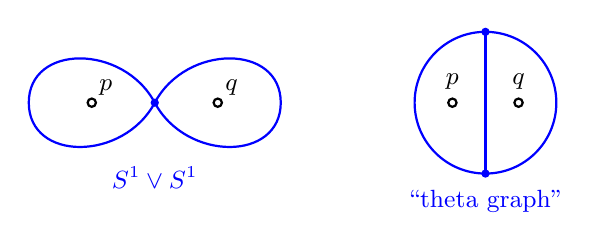
\begin{tikzpicture}[line width=0.8pt, every node/.style={font=\small}]
  % figure 8 = wedge of two circles, around the punctures p and q
  \draw[blue] (0,0) .. controls (-0.4,0.75) and (-1.6,0.75) .. (-1.6,0) .. controls (-1.6,-0.75) and (-0.4,-0.75) .. (0,0);
  \draw[blue] (0,0) .. controls (0.4,0.75) and (1.6,0.75) .. (1.6,0) .. controls (1.6,-0.75) and (0.4,-0.75) .. (0,0);
  \fill[blue] (0,0) circle (1.5pt);
  \draw (-0.8,0) circle (1.5pt) node[above right=-1pt] {$p$};
  \draw (0.8,0) circle (1.5pt) node[above right=-1pt] {$q$};
  \node[blue] at (0,-0.95) {$S^1\vee S^1$};
  % theta graph
  \begin{scope}[shift={(4.2,0)}]
    \draw[blue] (0,0) circle (0.9);
    \draw[blue] (0,0.9) -- (0,-0.9);
    \fill[blue] (0,0.9) circle (1.5pt) (0,-0.9) circle (1.5pt);
    \draw (-0.42,0) circle (1.5pt) node[above=1pt] {$p$};
    \draw (0.42,0) circle (1.5pt) node[above=1pt] {$q$};
    \node[blue] at (0,-1.25) {``theta graph''};
  \end{scope}
\end{tikzpicture}
